\documentclass[a4paper]{article}
\usepackage[utf8]{inputenc}
\usepackage[english]{babel}
\usepackage{microtype,etex,listings,color,parskip, graphicx, float}
\usepackage[margin=2cm]{geometry}
\usepackage[hidelinks]{hyperref}

\newcommand{\secref}[3][green]{\href{#2}{\color{#1}{#3}}}%
\newcommand{\urlref}[3][blue]{\href{#2}{\color{#1}{#3}}}%





\usepackage{wasysym}

\lstset{
    language=C,
    tabsize=2,
    showstringspaces=false,
    breaklines=true,
    basicstyle=\ttfamily,
    keywordstyle=\color[rgb]{0.1,0.3,0.7}\ttfamily,
    stringstyle=\color[rgb]{0.7,0.1,0.3}\ttfamily,
    commentstyle=\color[rgb]{0.3,0.4,0.3}\ttfamily,
    columns=fixed,
    numberstyle=\sffamily\scriptsize,
    backgroundcolor=\color[rgb]{0.95,0.95,0.95},
    frame=lines,
    framexleftmargin=5pt,
    numbers = left,
    numberstyle = \footnotesize,
}



\lstdefinelanguage{JS}{
    keywords={ var, typeof, new, true, false, catch,
        function, return, null, catch, switch, let, var, if, of, in,
    for, while, do, else, case, break, const},
    keywordstyle=\color{blue}\bfseries,
    ndkeywords={class, export, boolean, throw, implements, import, this},
    ndkeywordstyle=\color{darkgray}\bfseries,
    identifierstyle=\color{black},
    sensitive=false,
    comment=[l]{//},
    morecomment=[s]{/*}{*/},
    commentstyle=\color[rgb]{0.3,0.4,0.3}\ttfamily,
    stringstyle=\color{red}\ttfamily,
    morestring=[b]',
    morestring=[b]"
}

\lstset{
    language=JS,
    extendedchars=true,
    basicstyle=\footnotesize\ttfamily,
    showstringspaces=false,
    showspaces=false,
    numbers=left,
    columns=flexible,
    numberstyle=\tiny,
    numbersep=9pt,
    tabsize=2,
    breaklines=true,
    showtabs=false,
    captionpos=b,
}

\lstdefinelanguage{DPL}{
    keywords={ print, int, float, bool, var, typeof, new, true, false, catch,
        function, return, null, catch, switch, let, var, if, of, in,
    for, while, do, else, case, break, const},
    keywordstyle=\color{blue}\bfseries,
    ndkeywords={class, export, boolean, throw, implements, import, this},
    ndkeywordstyle=\color{darkgray}\bfseries,
    identifierstyle=\color{black},
    sensitive=false,
    comment=[l]{//},
    morecomment=[s]{/*}{*/},
    commentstyle=\color[rgb]{0.3,0.4,0.3}\ttfamily,
    stringstyle=\color{red}\ttfamily,
    morestring=[b]',
    morestring=[b]"
}

\lstset{
    language=DPL,
    extendedchars=true,
    basicstyle=\footnotesize\ttfamily,
    showstringspaces=false,
    showspaces=false,
    numbers=left,
    columns=flexible,
    numberstyle=\tiny,
    numbersep=9pt,
    tabsize=2,
    breaklines=true,
    showtabs=false,
    captionpos=b,
}

\begin{document}
\tableofcontents


\title{DPCC: DParo's Own C-Alike Compiler}
\author{Davide Paro}
\date{December 2020}

\maketitle

\section{Assignment Description}
This project is about an assignment for a course on \textbf{Compilers}
at the department of Computer Engineering Master Degree Padova (ITA).


The assignment consists in implementing a toy compiler for a toy language. More emphasis
is put on the implementation for the frontend side (input, lexing, parsing, type checking), while
the backend side is stubbed out by a simple 3AC \footnote{3AC: Three Address Code} Intermediate Code
generator.
We are free to design the syntax of this toy language however we like.

The assignment specs out the how the compiler should be composed.
We can in fact distinguish these macro components:

\begin{itemize}
\item \textbf{Input Stage} deals with the input byte stream that composes
    the source of the program.
\item \textbf{Lexer/Scanner} has the purpose of grouping characters (lexical analysis)
    together to compose compunded
    structures (called tokens). For the project assignment we can use \textbf{Flex} to aid in
    the implementation of the scanner.
\item \textbf{Parser} for performing the syntax analysis. It is what defines the look \& fell
    (grammar) of the language. For the project assignment we can use \textbf{Bison} to aid in the
    implementation of an LR parser.
\item \textbf{Intermediate Code Generator}. The ultimate purpose of a compiler is to produce something
    useful. In this project assignment we are not asked to implement a proper backend. Instead,
    we need to emit a 3AC representation of our input program. More in this later.
\end{itemize}

In particular the final Intermediate representation that we need to emit is based on Three Address Code (3AC),
that is, each statement can only have 1 operand at the left hand side of the assignment, and 2 operands at the right hand side
of the assignment, and an operator driving the operation that should be performed.

You can view more about 3AC at the following \urlref{https://en.wikipedia.org/wiki/Three-address_code}{Wikipedia link}.

In practice the emitted 3AC code is on itself a partially valid C program, it's only missing variable
declarations at the top for the temporary variables.


For the specification of the Intermdiate Code that is generated please refer to \hyperref[appendix_a]{appendix A}

So the project requires to produce this kind of 3AC / C hybrid. Control flow is allowed to be implemented
trough the usage of C labels and simple if conditional followed by a goto statement. Inside
the if conditional there can only be a single element composing the expression.

The assignment requires the following features from the programming langugage that we should develop:

\begin{itemize}
    \item Variables declaration, initialization and assignment
    \item Scoping. Variable names are reusable in different scopes. Variable
        shadowing may or may not warn/fail/pass depending on the design choices.
    \item Only 2 types of variables: integers, booleans
    \item Assignment statements, print statements, if statements, and at least 1 loop statement at our liking
    \item Handling of simple mathematical expressions that we can encounter in common programming
        languages: addition, subtraction, multiplication, division, modulo, etc \dots
    \item \textbf{Function definition, function calls, and custom user definable types are not required}
\end{itemize}

\clearpage

\section{DPL and dpcc: A quick peak at the language and at the compiler}

After describing the project assignment, from now on, the following sections will describe the proposed language
and the implemented compiler.

\textbf{DPL} and \textbf{DPCC} are respectively the \textbf{name of the language} and the
\textbf{name of the implemented compiler}. They are named after their author.

From now on \textbf{DPL} and \textbf{DPCC} will be used for brevity for refering to the language and to the compiler.
We will use \textbf{dpcc} (all lowercase) instead, to refer to the actual executable where the compiler lives.

That being said \textbf{DPCC} (all UPPERCASE) and \textbf{dpcc} (all lowercase) are mostly used interchangeably to refer to the same thing.


\subsection{DPL: Structure of the language}

\textbf{DPL} is mostly a C-alike compatible language, since it borrows most of its syntax and semantics.
It also borrows some syntax from \textbf{Rust} \&
\textbf{JS} especially in how the variables are declared (usage of the keyword \textbf{let}).

\textbf{Rust} is a modern system programming language with strong typing guarantees.
Among all the interesting features that Rust provides one of them is type deduction.
Thanks to Rust's strong typing guarantees and thanks to strong type deduction rules implemented
inside the \textbf{rustc} compiler, Rust
allows one to declare variables with a very low-weight syntax, similar
to a syntax provided from a typical dynamic language (for example JS).

\textbf{DPL}, like Rust, also have a very simple form of a type deduction system.
It is not even remotely close to the Rust type deduction system, but still it
allows the user of the language to not always need to specify the type of each variable in a declaration.
How this is achieved will be described in later sections.

In \textbf{DPL}:

\begin{itemize}
\item Spaces and newlines mostly do not matter, they simply introduce token boundaries.
\item Comments start with the double forward slash `\emph{//}', and C-style multiline comments are
instead not supported (at the time of writing).
\end{itemize}



Here follows some chunks of \textbf{DPL} code to show off the language concepts and syntax:

\begin{lstlisting}[language=DPL]
// Print statement with immediate C-style strings. C-style strings can only be used inside print statement
print("Hello world\n");

// Variable declaration and initialization
let a = 10;          // Integer Type deduced
let f = 10.0;        // Float type deduced
let b = false;       // Boolean type deduced

// Explicit types
let i: int = 0xffff & ~0xb00111;
let f: float = 10.0 + 20.0 ** 2;

// Immediate values can be printed
print(10);
print(30 + 4);

// Variables can be printed
print(i);       // Print integer
print(f);       // Print float

// Casting can be used to enforce type conversion
let myInt: int = int(10.00f);
let myFloat = float(0xFF);

// Type deduction
let b = (10 < 20);   // Boolean type is deduced
let f = 1 + 2.0f;    // Float type is deduced (the 1 is upcasted to a float)

// Scoping and restricting variable declarations to the current scope
{
    // Simple single dimension arrays declaration
    let buf_i: int[100];            // Known size integer array
    let buf_f: float[100];          // Known size float array

    // Integer array with deduced size from the RHS initializer list
    let buf = [ 10, 20, 30, 40, 50 ];

    // Arrays can be printed
    print(buf);
}

let buf: int[100];

// Control flow
for (let i = 0; i < 100; i++) {
    buf[i] = i ** 2;

    if (buf[i] == 10) {
        print("buf[i] is 10!!!\n")
    }
    else if (buf[i] == 20) {
        print("buf[i] is 20!!!\n");
    }
    else {
        print("None of above\n");
    }
}
\end{lstlisting}

The cool thing about \textbf{DPL}, is that it is \textbf{almost a Javascript subset}.
That is one can simply copy the \textbf{DPL} code, strip the type information (if they're used
anywhere) by manual editing or automatically, and paste the same code into a browser console to evaluate as JS code.
With a couple modifications here and there (for example arrays with no initalizer list must be converted into a valid
JS array), one can
test if the compiler \textbf{dpcc} is producing the correct output by simply
evaluating the same code in a browser console.

This example shows how to convert \textbf{DPL} into \textbf{JS} by manual editing:

\begin{lstlisting}[language=DPL]
// This is a chunk of DPLL code
let a = 10;                     // This is also valid JS code
let b = [ 10, 20, 30, 40 ];     // This is also valid JS code
let c: int = 10;                // Mostly valid JS code, remove the type info and the colon
let d: int[1024];               // Js arrays grow on demand automatically when touching elements.
                                // No need to specify neither type nor number of elements

print(d);                       // Valid JS code if function print were to be defined
\end{lstlisting}

Here's the equivalent JS code:

\begin{lstlisting}[language=JS]
// This is the equivalent Javascript
const print = console.log;      // Define it once at the top of the script

let a = 10;                     // Same as before
let b = [ 10, 20, 30, 40 ];     // Same as before
let c = 10;                     // Just strip the int type
let d = [];                     // Just initalize with empty array is enough

print(d);                       // Works because print is defined at the top
\end{lstlisting}

Most other \textbf{DPL} syntax and features, like code blocks, conditionals, loops \dots etc are valid JS code
thanks on how the grammar for \textbf{DPL} was defined.

For now \textbf{dpcc} supports only 5 types: \texttt{bool, int, float, string, bool[], int[], float[]}.
Only single dimensions array are for now supported. So arrays do not generalize to any number of dimensions.

Most of these types have full on semantics, meaning that the compiler can deduce
a type of an expression given the types of its operand. In some cases it can reject
the code if the operands of an expression have invalid types.
At the current time of writing this report, \texttt{string} types are quirky, meaning that
they don't have a full type tracking inside
the compiler like other types do.
The compiler still knows what a string is, and in it marks correctly \textbf{string literals} as
a \texttt{string} type, but strings undergo different semantics.
They cannot be assigned or operated on like a variable, but instead,
they can only be used as a parameter to the print statement.


\subsection{DPCC: Using the compiler}

The \textbf{dpcc} compiler is written in the \textbf{C} language. Unfortunately at the current time
of writing \textbf{dpcc} works only under Unix like operatins systems. The compiler has
been tested under Ubuntu 20.10, Ubuntu 20.04, and macOS 10.15. The
compiler was developed by his author using an Ubuntu 20.10 machine, while the other distro/OS
were tested thanks to Github Actions automated build-check cycles. Windows builds
failed due to MSVC rejecting the source code of \textbf{dpcc} cause it contains some GCC
extensions and some hard coded unix syscalls.
In short words \textbf{dpcc} can be only compiled with either GCC or CLANG compilers
and executed in a Unix/Posix compatible operating system.

If you would like to build the compiler yourself from scratch please refer to the \urlref{https://github.com/dparo/dpcc/wiki}{Project WIKI}\footnote{\urlref{https://github.com/dparo/dpcc}{Github Repo Link}}

The compiler can and should be invoked from the commandline. The \textbf{dpcc} executable
is self contained and doesn't reach for any implicit external asset and thus can be placed
anywhere in the system and invoked from anywhere.

From now on we assume the user has a fired up shell correctly \textbf{cd}-ed to the directory
holding the \textbf{dpcc} executable:

To call the compiler run the following command, which will print it's usage help message:

\begin{lstlisting}[language=Bash]
./dpcc
\end{lstlisting}

The \textbf{dpcc} compiler supports the specification of the \texttt{-o} flag
where applicable. This flag allows to override the default locations where
the compiler would produce it's output.

\textbf{dpcc} can work in 6 different modes: \textbf{lex, parse, 3ac, c, gcc, run}:

\begin{itemize}
    \item \texttt{./dpcc lex <input> [-o <out>]}: Lex the input and show the list of tokens composing the \textbf{DPL} source in either stdout or in the given file.
    \item \texttt{./dpcc parse <input> [-o <out>]}: Parse the program and produce a text representation of the AST (Abstract Syntax Tree) in either stdout or in the given file.
    \item \texttt{./dpcc 3ac <input> [-o <out>]}: Parse the program and perform additional type validations and type checking. If the program is still valid emit 3AC in either stdout or in the given file.
    \item \texttt{./dpcc c <input> [-o <out>]}: Same as 3AC but also emit preamble and postamble required  to promote 3AC to a  valid C program that can be compiled. The output is emitted in either stdout or in the given file.
    \item \texttt{./dpcc gcc <input> [-o <out>]}: Same as \texttt{`dpcc c'} but the generated C program is piped into GCC standard input and the final executable is either compiled in \texttt{a.out} or in the given filepath. This requires GCC to be in the path.
    \item \texttt{./dpcc run <input>}: Parse, typecheck, emit the C code, compile it and run it in one single command. The executable produced by GCC is outputted in a temp file (under \texttt{/tmp}), the temp executable is executed right away and then removed. The \texttt{-o} flag is ignored. This requires GCC to be in the path.
\end{itemize}

\texttt{Lex} and \texttt{parse} modes are mostly used for debugging and are not really that useful.
The \texttt{run} mode
is the most convenient mode since it takes care of everything. If the input program is valid and
you call \texttt{`./dpcc run'} on it you will see the output generated from you \textbf{DPL} program,
otherwise the compiler will complain with either warnings or errors.

\clearpage

\section{DPLL Language}


\dots \dots

\dots \dots Talk about how cool is this language \dots \dots

\dots \dots


\clearpage
\section{Implementation Details of the DPCC compiler}

In this section is briefly described the input stage, the lexer stage, and the syntax analysis stage (parser).

Talk about common types: ast_node_t, token_t and how they are mapped to the bison, flex equivalent.
How they are used and how they flow in the system. Explain that Bison is mostly used as a syntax
checker + symtable analysis, each node is defined and the pushed. Most complex type checking and
code generation steps are instead implemented somewhere else. Explain why you didn't implement
the necessary code right inside the bison grammar file.

\subsection{The input stage of the compiler}
This is the simplest part of the compiler. At the time of writing the \textbf{dpcc} compiler
allows only loading of files. In particular it reads an entire file into memory before continuining
with the rest of the piepeline. The input stage does not support URI, file downloads, any type of protocol
that would require realtime on stream code generation, and linux sockets. That is the
parser can open anything that looks like a file that has a finite determinable start, an end,
and a finite number of bytes.

\subsection{Lexer}

\urlref{https://github.com/westes/flex/}{Flex} is used to implement the lexer/tokenizer. Lexers are pretty simple to understand and
are particulary easy to develop if easing a tool like Flex. One can read the \urlref{https://www.cs.virginia.edu/~cr4bd/flex-manual/}{Flex Manual}.

The things that are worth noting about the \textbf{dpcc} tokenizer are:

\begin{itemize}
\item The lexer is completely UTF-8 aware, and UTF-8 symbols can be used to declare identifiers.UTF-8 aware and has particular
rules to match the variable encoding of UTF-8 \textbf{This allows variable names to include emojis}. Why? Cause it's cool \smiley
\item The lexer tracks line and column locations thanks to the \texttt{yylloc} exposed from bison. These
    variable is updated accordingly in the flex file whenever any token is encoutered the column information
    are updated and are resetted at each newline.
\item Support for C-style strings containing escape sequences.
\item Support for C-style single line comments
\item Support for binary and hexadecimal integers. Support for C-style floating point numbers with the exponent and optional terminating \texttt{`f'} character.
\item All the remaining tokens are pretty standard and uninstering.
\end{itemize}

This module is mostly un-interesting. Flex is used mainly as a token recognizer since most of the logic is implemented outside the flex
file anyway. One of the most notable feature that is implemented outside the lex file and used,
is what's called \textbf{String interning}\footnote{\urlref{https://en.wikipedia.org/wiki/String_interning}{String Interning Wikipedia Article}}.
\textbf{String iterning} is a common technique used in compilers design that allows the compiler to
store and cache lexemes in a common place. Since in typical source files
the same lexemes tend to repeat and appear multiple times, it is common to store each lexeme only once. Whenever
a lexeme is found it is looked up in a string to string hashmap. If it's not found, it allocates
the new lexeme and returns the pointer to the new allocation. If it's found instead, it simply just returns the pointer to the interned lexeme. This allows to save
memory, but even more cooler is the fact that now if two strings are identical and they are interned correctly,
we can compare the two strings for equality by simply just comparing their respective pointers. In fact
thanks to string interning strings are uniquely identified by the memory address they live in.
This feature is then used in the parser
to quickly lookup the identifiers in the symbol table.

So upon encountering a new token the following things happen:

\begin{itemize}
\item It updates correctly the state required in order to track the location of each token in the source file.
\item The lexeme is interned, and the old lexeme pointer is stomped in favour of the interned one.
\item It allocates a new \texttt{token\_t} and set's up the lexeme pointer, it's location and some other metadata
\item It allocates a \texttt{ast\_node\_t} and attaches the token to it. The \texttt{ast\_node\_t} is what will be
    used by Bison and later stages to generate the AST and to perform the analysis and the code generation.
\item It signals to bison the new lexeme kind by simply \texttt{return}-ing from the \texttt{lex()} procedure (Bison calls flex in a coroutine mode)
\end{itemize}

\subsection{Input stream based in read entire file into memory and then proceed. No realtime streaming, nor socket, etc...}

\subsection{Custom log is implemented to override default bison behaviour}

\subsection{Common types used withing the compiler}


\subsection{Most notable functions used in the compiler}

\subsection{How the AST is traversed}

\subsection{How type checking and type deduction is implemented}

\subsection{A brief introduction at the code implementing the compiler}

\begin{itemize}
    \item The order of the childs in each node \textbf{is very important} and it drives
        the correctness of the final output. In this way we can use simple printf to generate
        the code each time we find something while traversing the tree
\end{itemize}

\subsection{Typescript used for code generation of some part of the compiler}

\subsection{Encountered problems}

\subsection{Testing framework}

\section{Performance results}

\begin{figure}[H]
    \centering
    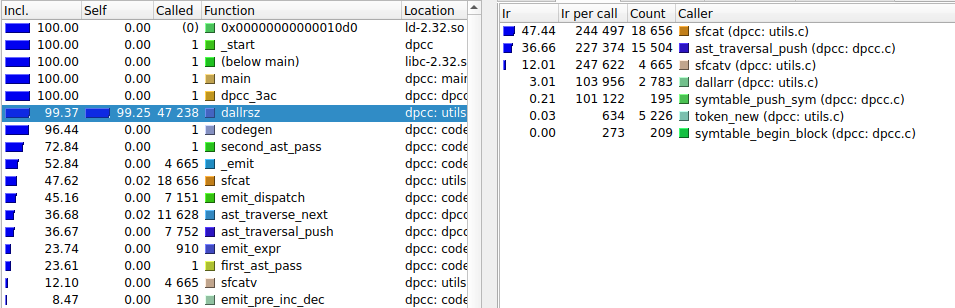
\includegraphics[width=\linewidth]{imgs/dallrsz_performance_issue.png}
    \caption{Performance issue in \texttt{dallrsz} utility function}
\end{figure}


\begin{figure}[H]
    \centering
    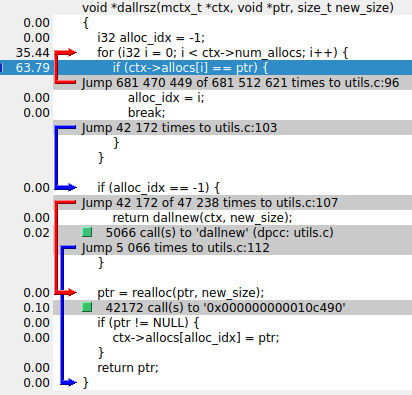
\includegraphics{imgs/dallrsz_code_usage.png}
    \caption{Performance issue in \texttt{dallrsz} utility function}
\end{figure}



\begin{figure}[H]
    \centering
    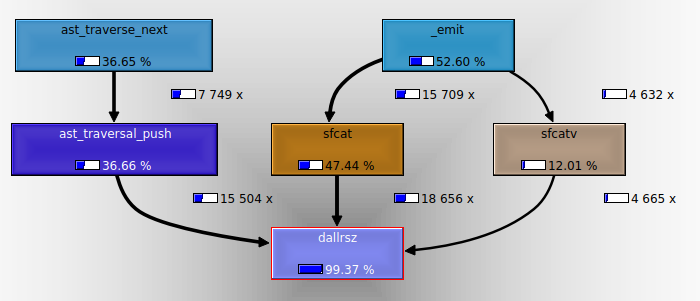
\includegraphics[scale=0.85]{imgs/dallrsz_callgraph.png}
    \caption{Performance issue in \texttt{dallrsz} utility function}
\end{figure}

\section{Problem analysis}

...

\section{Program design}

...

\section{Evaluation of the program}

...

% \section{Evaluation of the program} % Optional
%
% ...

\section{Process description}

...

\section{Conclusions}

...

\section{Appendix A: Structure of the Intermediate Code}
\label{appendix_a}

\section{Appendix: program text}

% Here you should include the program text.
% Do NOT use screenshots or similar methods.
% Below you can see how to use \lstinputlisting{}.



\begin{lstlisting}[language=DPL]
let a: int[] = 10;
let s = "Hello world";
{

}
\end{lstlisting}

\begin{lstlisting}[language=C]
int main() {

}
char **argv;
\end{lstlisting}


\clearpage
\section{Appendix B: Example Program Iterative Merge Sort}
\label{appendix_b}

\begin{lstlisting}[language=DPL]
let len = 32;

let array = [
    15, 59, 61, 75, 12, 71,  5, 35, 44,
    6, 98, 17, 81, 56, 53, 31, 20, 11,
    45, 80,  8, 34, 71, 83, 64, 28,  3,
    88, 50, 48, 80,  5
];


for (let cs = 1; cs < len; cs = 2 * cs) {
    for (let l = 0; l < len - 1; l = l + 2 * cs) {
        let m = len - 1;

        if ((l + cs - 1) < len - 1) {
            m = l + cs - 1;
        }

        let r = len - 1;

        if ((l + 2 * cs - 1) < len - 1) {
            r = l + 2 * cs - 1;
        }

        let n1 = m - l + 1;
        let n2 = r - m;

        let L: int[1024];
        let R: int[1024];

        for (let i = 0; i < n1; i++) {
            L[i] = array[l + i];
        }

        for (let i = 0; i < n2; i++) {
            R[i] = array[m + 1 + i];
        }


        let i = 0;
        let j = 0;
        let k = l;

        while (i < n1 && j < n2) {
            if (L[i] <= R[j]) {
                array[k++] = L[i++];
            } else {
                array[k++] = R[j++];
            }
        }

        while (i < n1) {
            array[k++] = L[i++];
        }
        while (j < n2) {
            array[k++] = R[j++];
        }
    }
}

print("Sorted array\n");
print(array);
\end{lstlisting}


% \section{Appendix: test cases} % Optional
%
% ...

% \section{Appendix: Extensions} % Optional
%
% ...

\end{document}
